\documentclass[a4paper,10.5pt]{report}
\usepackage[top=2.5cm,bottom=3cm,right=3cm,left=3cm]{geometry}
\usepackage[utf8]{inputenc}
\usepackage[T1]{fontenc}
\usepackage[english]{babel}
\usepackage{graphicx,graphics,textcomp,setspace,lettrine}
\usepackage{amsmath,amssymb,amsfonts,indentfirst}
\usepackage[toc,page]{appendix}
\usepackage{float}
\usepackage{array}
\usepackage{comment}
\usepackage{xcolor}
\usepackage{listings}
\usepackage{blindtext}
\usepackage{titling}
\usepackage{multicol}
\usepackage{enumitem}
\usepackage{ulem}
\usepackage{cancel}
\usepackage{wasysym}
\usepackage{hyperref}
\usepackage{gensymb}
\usepackage{listings}


\graphicspath{{plot/}}

\newcommand{\cfbox}[2]{%
    \colorlet{currentcolor}{.}%
    {\color{#1}%
    \fbox{\color{currentcolor}#2}}%
}

\usepackage[english, status=draft]{fixme}
\fxusetheme{color}

\lstset{numbers=left,
numberstyle=\tiny \bf ,
stepnumber=1,
numbersep=10pt,
firstnumber=1,
numberfirstline=true}

\lstset{frame=TBlr,
rulesepcolor=\color{black}}

\DeclareMathOperator{\e}{e}

\usepackage{fancyhdr}
\pagestyle{fancy}

\renewcommand{\headrulewidth}{1pt}
\fancyhead[L]{\leftmark}
\fancyhead[R]{}

\renewcommand{\footrulewidth}{1pt}
\fancyfoot[C]{\textbf{\thepage}}
\fancyfoot[L]{}

\title{{\textsc{\Large{TP General Physics / M1}\\ [3cm]
      \textbf{\LARGE{High Velocity Cloud Analysis \\ in \\ HI4PI Data}}}} \\[2cm]}
\vfill
 \author{Antoine Marchal \\
 updated by Louis Legrand \\ [1cm]
Université Paris-Sud \\
Institut d’Astrophysique Spatiale \\
2019-2020}
\date{}


\begin{document}
\begin{titlingpage}
\maketitle
\end{titlingpage}
%% \tableofcontents
\newpage

\newpage
\chapter{Introduction}
The study of our own galaxy, the Milky Way, is complicated by the fact that we are within it.
The sun, located at 8.5 kpc from the galactic center, moves in a circular orbit with a radial velocity of
220 km.s$^{-1}$.
As a first approximation, we can discribe the galactic plane as a sum of three components : Gas (molecular and neutral hydrogen), Star
and Dark Matter. Around this galactic plane, in what is called the galactic halo, there is an important gas reservoir mainly composed of neutral gas (HI).
It turns out that this reservoir could be an important source of gas for the formation of molecular clouds, the place where stars are formed.
To better understand the content and nature of this reservoir, we propose in this work to study one of these clouds, called High Velocity Clouds (HVC).

\begin{figure}[h!]
  \centering
  \includegraphics[width=0.5\textwidth]{simulation.png}
  \label{fig::simulation}
  \caption{(a) Integrated intensity, (b) centroid velocity, and (c) velocity dispersion of a model CHVC (model Wb1a15b of
    Heitsch \& Putman (2009)), traveling at 45\,\degree{} to the observer. Contours are given at [1, 5, 9, 13] K km s-1.
    (from Heitsch et al, 2016)}
\end{figure}

Since their discorevy by Muller et al (1963), High Velocity Clouds are studied as isolated objects. They are defined
as HI clouds with a radial velocity (typically $ V_r \approx 200 \, km.s^{-1}$) that cannot be explained by the rotation
curve of the Milky Way (Wakker 1991). Figure~\ref{fig::simulation} shows an HVC view from a numerical simulation performed by
Heitsch et al, 2016. HI is observed since many years through the 21 cm hyperfine structure line, and the latest full sky survey
has been released by the HI4PI collaboration. More details are present in this recent article :
\color{blue} \url{https://arxiv.org/abs/1610.06175} \color{black}.
The research project we adress here is based on a single HVC cloud named HVC125+41-207.
Starting from a part of this survey, we develop a simple method to obtain some physical properties of this cloud
and its environment. \\

To download the data cube from HI4PI:


\verb|wget http://cdsarc.u-strasbg.fr/ftp/J/A+A/594/A116/CUBES/GAL/CAR/CAR_G07.fits|
% \begin{lstlisting}
% wget http://cdsarc.u-strasbg.fr/ftp/J/A+A/594/A116/CUBES/GAL/CAR/CAR_G07.fits
% \end{lstlisting}


\newpage
\noindent
\underline{Physical constants} : \\
\begin{itemize}
\item[$\bullet$] Atomic mass of hydrogen : $m_H = 1.6737236 \times 10^{-27} \, kg$
\item[$\bullet$] Definition of a parsec : $pc = 3.085677581467192 \times 10^{16} \, m$
\item[$\bullet$] Mass of the Sun : $M_{\astrosun} = 1.9891 \times 10^{30} \, kg$
\item[$\bullet$] Mean mass per particle within the sphere : $\mu \approx 1.25 \, m_H$
\item[$\bullet$] Boltzmann constant : $k = 1.38064852 \times 10^{-23} \, m^2.kg.s^{-2}.K^{-1}$
\end{itemize}

%% \addcontentsline{toc}{chapter}{Introduction}
\chapter{Getting started - hyperspectral cube}
\section{Reading Data from FITS Files}
This work is based on an hyperspectral observation of the 21 cm line
(see representation figure~\ref{fig::hyperspectral}). For each line of sigh across the observation, a simple Doppler effet
calculation allows us to obtain a projected velocity spectrum. \\

\begin{figure}[h!]
  \centering
  \includegraphics[width=3.in]{hyperspectral.pdf}
  \label{fig::hyperspectral}
  \caption{3D representation of a hyperspectral cube. All the points on a straight line in this cube compose a spectrum.
  We can select a sub-regoin of this cube which corresponds to a smaller part of the sky.}
\end{figure}

We propose to read this hyperspectral observation formatted in FITS using python.
A good documentation is available via the following link:
\color{blue} \url{http://docs.astropy.org/en/stable/io/fits/} \color{black}

\section{High Velocity Cloud location}
To understand the data we are using, a first exercice would be to visualize the total integreted column density map of the field
using Eq. \ref{eq::NHI}. There is no clear evidence of an HVC in this map, simply because the total integrated density is dominated
by the HI emission of the Milky Way. Indeed, the HVC HVC125+41-207 is located in the following spectral range : $v_{rad} (km.s^{-1}) = [-225, -185]$.
From the article describing the HI4PI survey, it is also possible to clean the cube considering the rms value. For exemple we can keep
all values greater than $3 \times \sigma_{rms}$, with $\sigma_{rms}$ the sensitivity of the radio telescope used.


After selecting the spectral range, we can plot the HVC using the 'imshow' function of matplotlib
(see \color{blue} \url{http://matplotlib.org} \color{black}) \\
Note that the galactic longitude range and the galactic latitude range of the cube are respectively
$l(deg) \in [119, 141]$ and $b(deg) \in [19, 51]$.

\begin{figure}[h!]
  \centering
  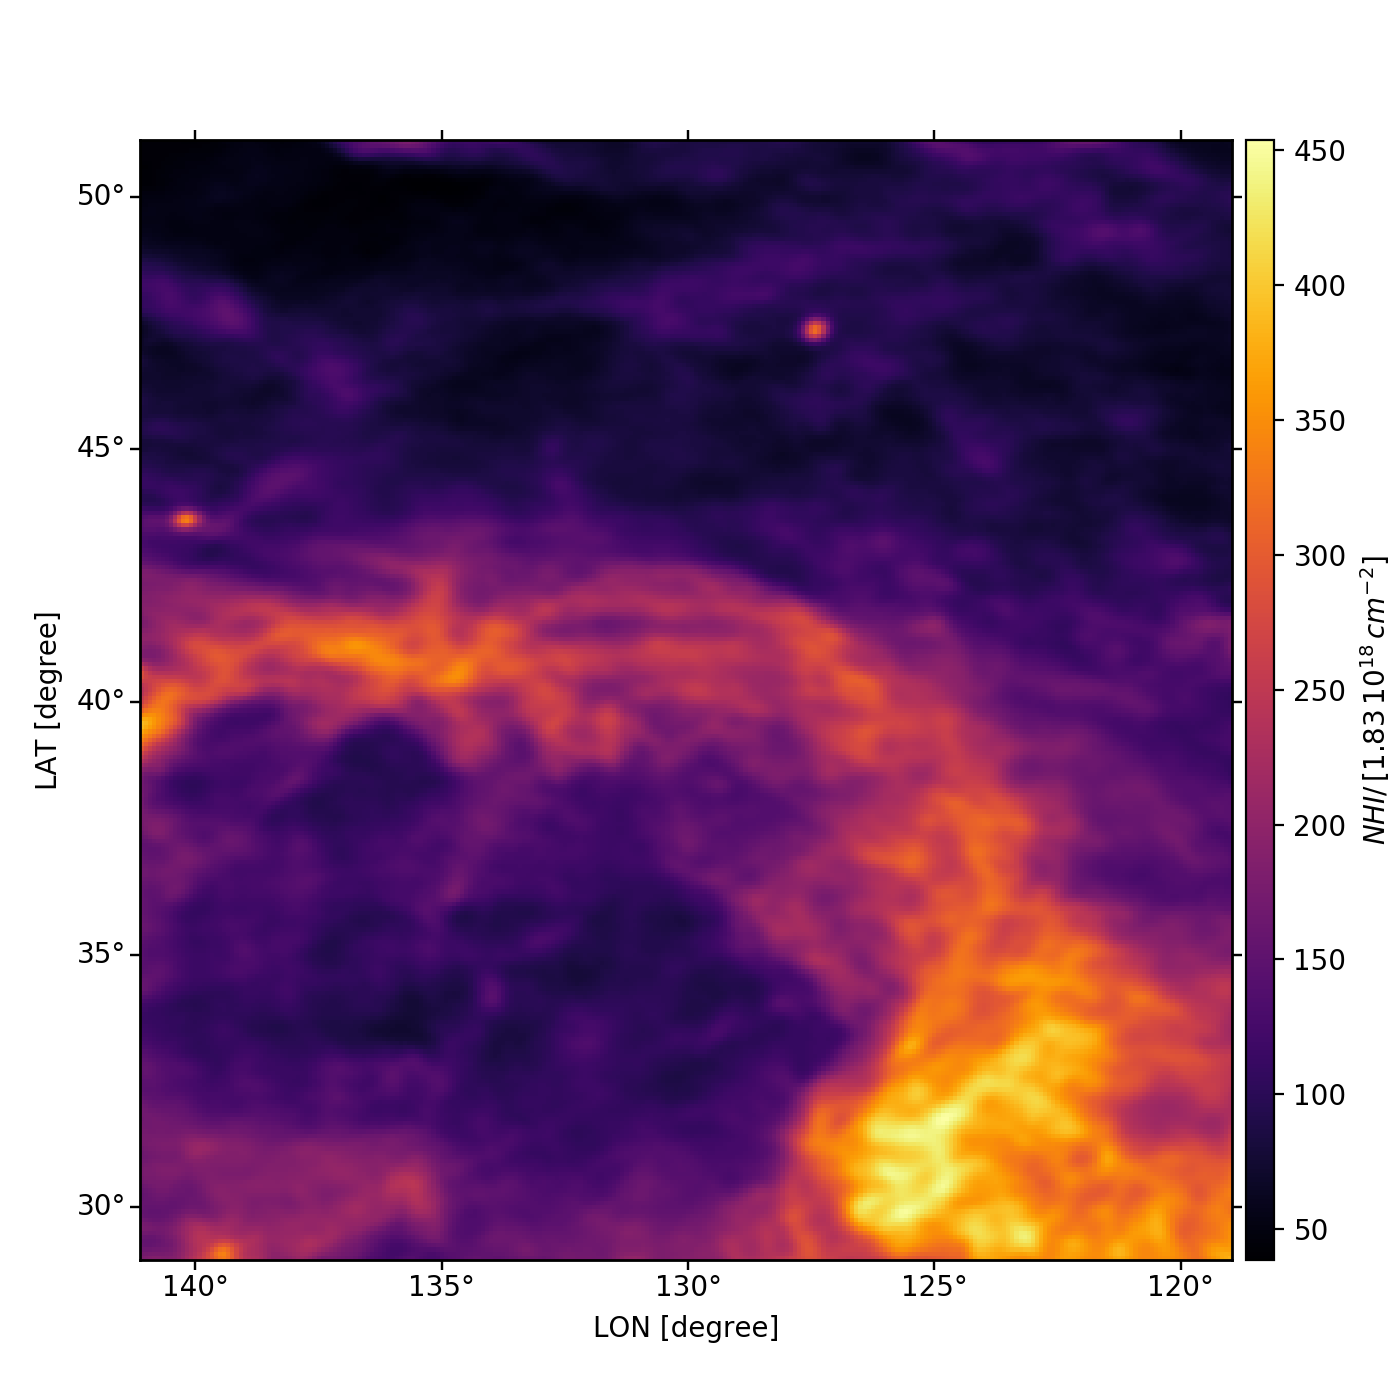
\includegraphics[width=3.5in]{field.png}
  \label{fig::hyperspectral}
  \caption{Total integreted column density map of the field. Note that the coordinates are in the galactic coordonate system.}
\end{figure}

\begin{figure}[h!]
  \centering
  \includegraphics[width=3.5in]{hvc_select.png}
  \label{fig::hvc}
  \caption{Integrated intensity map of HVC125+41-207 High Velocity Cloud, i.e integration perform in the velocity range of the cloud.}
\end{figure}

\chapter{Physical properties of the HVC}
\section{Mean spectra of the HVC}
To obtain some physical properties of this clump, we can analize the mean spectrum of the HVC.
Figure~\ref{fig::spectra} shows a schematic view of the numerical calculation required to obtain the average spectrum of the cloud
from the hyperspectral cube.

\begin{figure}[h!]
  \centering
  \includegraphics[width=6.in]{spectra.png}
  \label{fig::spectra}
  \caption{Representation of the passage of hyperspectral data to the mean spectrum of the cloud}
\end{figure}

\section{Spectral analysis}
As a first approximation, we can applied the Virial equilibrium to obtain the pressure outside the HVC as a function
of the distance d (preferentialy expressed in kpc which is a unit of length used in astronomy).
It is nothing more than the balance between the inner and outer medium.

\begin{align}
  \frac{P_s}{k} = \underbrace{\frac{\left< N_{HI} \right> \, T_k}{d \, \theta}}_\text{kinetic pressure} \,
  \underbrace{- \, \frac{\mu^2 \, G \, \pi \, \left< N_{HI} \right>^2}{15 \, k}}_\text{gravitational pressure}
\end{align}
where $\theta$ is the observed angular diameter in radian, $T_k$ is the kinetic temperature of the gas, d is the distance of the clump,
$G$ and $k$ and respectively the gravitational constant and the Boltzmann constant, $\left< N_{HI} \right>$ is the mean value
of the column density and $\mu$ the mean mass per particle within the sphere. \\

\noindent From the average sprectrum of the clump, we can estimate the mean integrated column density
$\left< N_{HI} \right>$ from 21 cm measurements. \\
\begin{align}
  \frac{\left< N_{HI} \right>}{cm^{-2}} = 1.82243 \times 10^{18} \times \int_{-\infty}^{+\infty} \left( \frac{T_b(v)}{K} \right)
  d\left( \frac{v}{km.s^{-1}}\right)
  \label{eq::NHI}
\end{align}
where $T_b$ is the mean brightness temperature and $dv$ is the spectral resolution. \\

\noindent Note that we can direclty obtain the surface density :
\begin{align}
  \Sigma = \frac{\left<N_{HI}\right> \, m_H \, pc^2}{M_\odot}
\end{align}
where $m_H$ is the atomic mass of hydrogen, $pc$ is the definition of a parsec,
and $M_{\astrosun}$ is the mass of the Sun. \\

Considering that the observed velocity dispersion is only due to the thermal broadening, the kinetic temperature
of our system $T_k$ can be written as :
\begin{align}
  T_k = \frac{m_H \, \sigma_v^2}{k} \, (K)
\end{align}
$\sigma_v$ is computed by fitting a Gaussian function on the average spectrum obtained previously.

\newpage
%\listoffixmes
\end{document}

